\section{Reock}\label{sec:reock}

Let $\mathrm{circ}(\Omega)$ denote the \textit{smallest bounding
circle} (smallest bounding \textit{cap} on the sphere) of a region
$\Omega$.  Then the \textit{Reock score} of $\Omega$ is 

$$\mathrm{Reock}(\Omega)=
\frac{\mathrm{area}(\Omega)}{\mathrm{area}(\mathrm{circ}(\Omega))}.$$

We again consider what properties a map projection $\vphi$ must have in order to preserve the ordering of regions by their Reock scores.  
\zs{add discussion about the use of this score, why it's good, why not}
\begin{lemma}\label{lem:reock_prep}
  If $\vphi$ preserves the ordering of regions induced by their convex hull scores, then the following must hold:
  \begin{enumerate}
    \item $\vphi$ sends spherical caps in its domain to Euclidean circles in the plane,  and $\vphi^{-1}$ does the opposite 
    \item There exists a region $U$ in the domain of $\vphi$ such that for any regions $A,B\subset U$, if $A$ and $B$ have equal area on the sphere, then $\vphi(A)$ and $\vphi(B)$ have equal area in the plane.  The same holds for $\vphi^{-1}$ for all pairs of regions inside of $\vphi(U)$.
  \end{enumerate}
\end{lemma}
\begin{proof}
  Similarly to the convex hull setting, the proof of (1) follows from the requirement that $\vphi$ preserves the maximizers in the compactness score ordering.  In the case of the Reock score, the maximizers are caps in the sphere and circles in the plane.

  

  To show (2), let $\kappa$ be a cap in the domain of $\vphi$, and let 
  $A,B\subset \kappa$ be two regions of equal area properly contained in the interior of
  $\kappa$. Then, define two new regions $X=\kappa\ssm A$ and $Y=\kappa\ssm B$, which can be 
  thought of as $\kappa$ with $A$ and $B$ deleted, respectively. 
  
  Since $\kappa$ is the smallest bounding cap of $X$ and $Y$ and since $A$ and $B$ have equal areas, $\mathrm{Reock}(X)=\mathrm{Reock}(Y)$.  Furthermore, by (1), $\vphi$ must send $\kappa$ to some circle in the plane, 
  which is the smallest bounding circle of $\vphi(X)$ and $\vphi(Y)$.    
  Since $\vphi$ preserves the ordering of Reock scores, it must be that $\vphi(X)$ and $\vphi(Y)$ have identical Reock 
  scores in the plane.
  
  By definition, we have
  \begin{align*}
  \mathrm{Reock}(X) &= \mathrm{Reock}(Y)\\
  \frac{\mathrm{Area}(\vphi(X))}{\mathrm{Area}(\vphi(\kappa))} &= \frac{\mathrm{Area}(\vphi(Y))}{\mathrm{Area}(\vphi(\kappa))}
  \end{align*}
  and by the construction of $X$ and $Y$, we have 
  \begin{align*}
  \frac{\mathrm{Area}(\vphi(\kappa)) - \mathrm{Area}(\vphi(A))}{\mathrm{Area}(\vphi(U))} &= \frac{\mathrm{Area}(\vphi(\kappa)) - \mathrm{Area}(\vphi(B))}{\mathrm{Area}(\vphi(\kappa))}\\
  \mathrm{Area}(\vphi(A)) &= \mathrm{Area}(\vphi(B)),
  \end{align*}
  
  
\mute{  
  \begin{align*}
    \mathrm{Reock}(X) 
    = 1-\frac{\mathrm{Area}(A)}{\mathrm{Area}(\kappa)} 
    = 1-\frac{\mathrm{Area}(B)}{\mathrm{Area}(\kappa)}
    = \mathrm{Reock}(Y)
  \end{align*}
  Note that $\kappa$ is sent to a circle in the plane, so 
  the minimal bounding circle of $\vphi(\kappa)$ is itself. Thus, 
  since $\vphi$ preserves equality of Reock scores,
  \begin{align*}
    1-\frac{\mathrm{Area}(\vphi(A))}{\mathrm{Area}(\vphi(\kappa))} 
    = \mathrm{Reock}(\vphi(X)) 
    = \mathrm{Reock}(Y)
    = 1-\frac{\mathrm{Area}(\vphi(B))}{\mathrm{Area}(\vphi(\kappa))}
  \end{align*}
  
}
  
  meaning that $\mathrm{Area}(\vphi(A) = \mathrm{Area}(\vphi(B))$. 
  Thus, for all pairs of regions of the same area inside of $\kappa$, the images 
  under $\vphi$ of those regions will have the same area as well.
  
  The same construction works in reverse, which demonstrates that  $\vphi^{-1}$ also sends 
  regions of equal area in some circle in the plane to regions of  equal area in the sphere.
  
 \end{proof} 



We can now show that no such $\vphi$ exists.  Rather than constructing a figure on the sphere and examining its image under $\vphi$, it will be more convenient to construct a figure in the plane and reason about $\vphi^{-1}$.
 
\begin{theorem}\label{thm:reockbad}
  There does not exist a map projection with the two properties in \Cref{lem:reock_prep}.
\end{theorem}
\begin{proof}
	
	Assume that such a $\vphi$ does exist and restrict its domain to a cap $\kappa$ as above.  This corresponds to a restriction of the domain of $\vphi^{-1}$ to a circle in the plane.  Inside of this circle, draw seven smaller circles of equal area tangent to each other as in \Cref{fig:sevencircles}.
	
	
	
  \begin{figure}[!htb]
	\label{fig:sevencircles}
	
	\centering

	
\begin{tikzpicture}[scale=.5,line cap=round,line join=round,>=triangle 45,x=1cm,y=1cm]
\clip(-11.346776859504123,1.0846280991735546) rectangle (9.810247933884293,16.026776859504118);
\draw [line width=2.1pt] (-2.6746410161513783,12.872407940936126) circle (2.4400204917172323cm);
\draw [line width=2.1pt] (-5.097320508075692,8.636203970468065) circle (2.4400204917172315cm);
\draw [line width=2.1pt] (-2.64,4.42) circle (2.440020491717234cm);
\draw [line width=2.1pt] (2.24,4.44) circle (2.4400204917172372cm);
\draw [line width=2.1pt] (4.662679491924313,8.676203970468062) circle (2.440020491717239cm);
\draw [line width=2.1pt] (2.2053589838486225,12.892407940936126) circle (2.4400204917172372cm);
\draw [line width=2.1pt] (-0.21732050807568942,8.656203970468063) circle (2.4435284258377075cm);
\draw [line width=1pt] (-2.6746410161513783,12.872407940936126)-- (-0.21732050807568942,8.656203970468063);
\draw [line width=1pt] (-0.21732050807568942,8.656203970468063)-- (2.2053589838486225,12.892407940936126);
\draw [line width=1pt] (2.2053589838486225,12.892407940936126)-- (-2.6746410161513783,12.872407940936126);
\draw [line width=1pt] (-2.6746410161513783,12.872407940936126)-- (-5.097320508075692,8.636203970468065);
\draw [line width=1pt] (-5.097320508075692,8.636203970468065)-- (-2.64,4.42);
\draw [line width=1pt] (-2.64,4.42)-- (2.24,4.44);
\draw [line width=1pt] (2.24,4.44)-- (4.662679491924313,8.676203970468062);
\draw [line width=1pt] (4.662679491924313,8.676203970468062)-- (2.2053589838486225,12.892407940936126);
\draw [line width=1pt] (4.662679491924313,8.676203970468062)-- (-0.21732050807568942,8.656203970468063);
\draw [line width=1pt] (-0.21732050807568942,8.656203970468063)-- (2.24,4.44);
\draw [line width=1pt] (-0.21732050807568942,8.656203970468063)-- (-2.64,4.42);
\draw [line width=1pt] (-0.21732050807568942,8.656203970468063)-- (-5.097320508075692,8.636203970468065);
\begin{scriptsize}
\draw [fill=black] (-2.64,4.42) circle (4pt);
\draw [fill=black] (2.24,4.44) circle (4pt);
\draw [fill=black] (4.662679491924313,8.676203970468062) circle (4pt);
\draw [fill=black] (2.2053589838486225,12.892407940936126) circle (4pt);
\draw [fill=black] (-2.6746410161513783,12.872407940936126) circle (4pt);
\draw [fill=black] (-5.097320508075692,8.636203970468065) circle (4pt);
\draw [fill=black] (-0.21732050807568942,8.656203970468063) circle (4pt);
\end{scriptsize}
\end{tikzpicture}

	\caption{Seven circles arranged as in the construction for \Cref{thm:reockbad}.}
\end{figure}	
	
\mute{
  \begin{figure}[!htb]
  	\label{fig:sevencircles}
  \begin{center}
    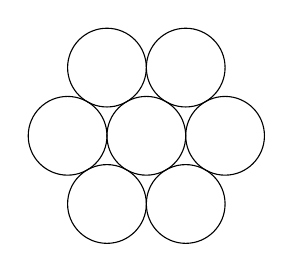
\begin{tikzpicture}
      \draw (0,0) circle (0.5);
      \draw (1,0) circle (0.5);
      \draw ({cos(60)},{sin(60)}) circle (0.5);
      \draw ({cos(120)},{sin(120)}) circle (0.5);
      \draw ({cos(180)},{sin(180)}) circle (0.5);
      \draw ({cos(240)},{sin(240)}) circle (0.5);
      \draw ({cos(300)},{sin(300)}) circle (0.5);
    \end{tikzpicture}
  \end{center}
\caption{Seven circles arranged as in the construction for \Cref{thm:reockbad}.}
\end{figure}


  Under $\vphi^{-1}$, they must be sent to an similar configuration 
  of equal-area caps on the sphere .  
  
  However, the radius of a
  of a spherical cap is determined by its area, so since the areas of these caps
  are all the same, their radii must be as well. Thus, 
  the midpoints of these caps form six equilateral triangles on the sphere
   which meet at a point.  However, this is impossible, as the three 
  angles of an equilateral triangle on the sphere must all be greater than $\tfrac{\pi}{3}$, 
  but the total measure of all the angles at a point must be equal to $2\pi$, which contradicts 
  the assumption that such a $\vphi$ exists.
\end{proof}

This shows that no map projection exists which preserves the ordering of regions by their Reock scores.
